\documentclass[11pt]{article}
\usepackage[utf8]{inputenc}
\usepackage[spanish,es-tabla]{babel}  % \decimalpoint %dejar de comentar si punto para decimales

\usepackage[unicode]{hyperref} % cargar casi al final
\hypersetup{
  colorlinks=true,
  urlcolor=blue,
  linkcolor=black,
  citecolor=black,
  breaklinks=true
}
\usepackage{url}
\usepackage{graphicx}
\usepackage{geometry}
\usepackage{multirow}
\usepackage{listings}
\usepackage[toc,page]{appendix}
\usepackage[spanish]{cleveref}
\usepackage{float}
\usepackage{booktabs}
\usepackage{multicol}
\usepackage{caption}   % para \captionof



\usepackage{xcolor}

\definecolor{codegreen}{rgb}{0,0.6,0}
\definecolor{codegray}{rgb}{0.5,0.5,0.5}
\definecolor{codepurple}{rgb}{0.58,0,0.82}
\definecolor{backcolour}{rgb}{1,1,1}

\lstset{
backgroundcolor=\color{backcolour},   
commentstyle=\color{codegreen},
keywordstyle=\color{magenta},
numberstyle=\tiny\color{codegray},
stringstyle=\color{codepurple},
basicstyle=\small\ttfamily,
breakatwhitespace=false,   
keepspaces=true,
showstringspaces=false,
columns=flexible,
breaklines=true,
inputencoding=utf8,
extendedchars = true  % Extended ASCII
} 

\geometry{a4paper, left=20mm, right=20mm, top=20mm, bottom=20mm}
\renewcommand{\listtablename}{Lista de tablas}
\renewcommand{\tablename}{Tabla}
\renewcommand{\lstlistingname}{Algoritmo}% Listing -> Algorithm
\renewcommand{\lstlistlistingname}{Lista de \lstlistingname s}% List of Listings -> List of Algorithms






\begin{document}

\begingroup
\tiny % \small in 11pt base font is 10pt
\begin{frame}
\\	\centering
	\resizebox{\textwidth}{!}{
%%%%	{\fontsize{20}{25} \selectfont}
	\begin{tabular}{c c} \hline
	\multirow{5}{*}{$\vcenter{\hbox{
\includegraphics[width=1.5cm]{./anexos/isologotipo-para-fondo-blanco.png}}}$} 
	& UNIVERSIDAD TECNOLÓGICA DEL URUGUAY\\
	& ITR SUROESTE $\cdot$ FRAY BENTOS\\
	& INGENIERÍA MECATRÓNICA \\
	& UC de Programación IV $\cdot$ 2022/2\\
	& Profesor: Giovani Bolzan Cogo \\		\hline
	\end{tabular}} \\
	\resizebox{\textwidth}{!}{
	\begin{tabular}{l |rr} 
	\multirow{2}{*}{Práctico de laboratorio II - Programación Orientada a Objetos} & \multirow{2}{*}{Periodo:}
	&de 19/09/2025\\	\cline{3-3}
	& &hasta 03/10/2025\\	\hline 
	\end{tabular}}
\end{frame}
\endgroup
%%%%%%%%%%%%%%%%%%%%%%%%%%%%%%%%%%%%%%%%%%%%%%%%%%%%%%%%%%%%%%%%%%%%%%%%%%%%%%%%%%%%
%%%%%%%%%%%%%%%%%%%%%%%%%%%%%%%%%%%%%%%%%%%%%%%%%%%%%%%%%%%%%%%%%%%%%%%%%%%%%%%%%%%%

%%%%%%%%%%%%%%%%%%% grupo de estudiantes %%%%%%%%%%%%%%%%%%%%%
\begin{flushright}
\subsection*{Integrantes}
	\subitem Felipe Morrudo -- 5.582.493-4
	\subitem Hector Pereira -- 5.582.582-5
        \subitem Santiago Moizo -- 5.165.430-5
        \subitem Aldrin Pacheco --
\end{flushright}
%%%%%%%%%%%%%%%%%%%%%%%%%%%%%%%%%%%%%%%%%%%%%%%%%%%%%%%%%%%%%%

\begin{abstract}
    Este trabajo implementa un sistema de gestión de clientes, vendedores, productos y compras usando Programación Orientada a Objetos en Python. El diseño se documenta con un diagrama de clases UML donde se modelan las relaciones clave: composición entre Compra e ItemCompra, y asociación/agregación con Producto, además de los vínculos con Cliente y Vendedor. La persistencia se resuelve con archivos de texto en formato JSON Lines (un registro por línea), con escritura atómica para evitar corrupción y funciones de carga que reconstituyen instancias a partir de índices por código. Se desarrolló un menú de consola para crear, listar y borrar entidades y para registrar compras con varios ítems, calculando totales y almacenando metadatos de factura. Los resultados muestran que el guardado/carga es consistente y que el modelo es extensible para incorporar validaciones adicionales, descuentos e impuestos.
\end{abstract}

\newpage
\tableofcontents
\newpage

\section{Introducción}

El presente informe documenta el desarrollo de un sistema de gestión de clientes, vendedores, productos y compras, implementado en Python bajo el paradigma de Programación Orientada a Objetos (POO). El trabajo corresponde al Práctico de Laboratorio II y aplica de forma integrada modelado con UML, diseño de clases y persistencia en archivos de texto.

El proyecto se apoya en un diagrama UML que describe las entidades principales y sus relaciones (composición entre Compra e ItemCompra, y asociaciones con Cliente, Vendedor y Producto). Este modelo guió la implementación, definiendo responsabilidades, encapsulamiento y navegación entre objetos.

Para la persistencia se utilizó el formato JSON Lines (JSONL), que almacena cada registro en una línea independiente y facilita la escritura y lectura incremental. Se desarrollaron funciones genéricas para serializar y rehidratar instancias, manteniendo consistencia entre modelo y datos en disco.

El informe presenta los objetivos, la fundamentación teórica, la metodología de desarrollo, los resultados (incluyendo UML final y evidencias de ejecución) y una discusión de conclusiones y posibles mejoras.


\section{Objetivos}
Este práctico tiene como objetivo general el modelado Orientado a Objetos (O.O.) de un sistema de gestión de ventas de una empresa ficticia, aplicando análisis de estructuras de datos y modelado en diagrama UML (Unified Modeling Language).

De los objetivos puntuales, destácanse los siguientes.
\begin{itemize}
    \item Modelar el dominio con clases y relaciones UML consistentes con el código.
    \item Implementar persistencia en archivos TXT usando JSONL con escritura atómica.
    \item Proveer un menú de consola para crear, consultar y borrar entidades y registrar compras.
    \item Rehidratar objetos desde disco con funciones \texttt{load\_*} e índices por código para resolver referencias.
\end{itemize}


\section{Fundamentación teórica} \label{fundamentos}

El desarrollo del código se realiza en Python, un lenguaje de sintaxis clara y modelo de objetos uniforme. Su tipado dinámico con anotaciones opcionales facilita documentar expectativas y expresar reglas de negocio de forma directa, apoyándose en una amplia biblioteca estándar para manejo de archivos, datos y ejecución sin agregar complejidad innecesaria.

\subsection{Fechas y tiempos}

\paragraph{\textbf{\textit{dateutil.parser}}} aporta un analizador flexible de fechas capaz de reconocer múltiples formatos habituales sin configuraciones extensas.
\paragraph{\textbf{dateparser}} complementa lo anterior al interpretar expresiones en lenguaje natural  (“hoy”, \linebreak “mañana”, “15/03/25”), reduciendo errores de carga y normalizando la información temporal en objetos datetime comparables y ordenables.

\subsection{Datos en archivos de texto}
Con \textbf{\textit{json}} se guardan y leen listas, diccionarios, números y textos en un formato estándar. Esto facilita almacenar el estado del sistema, recargarlo posteriormente o intercambiar datos con otras herramientas.

\subsection{Rutas y archivos}
\textbf{\textit{pathlib.Path}} permite trabajar con rutas como objetos (no como simples cadenas). Así podemos preguntar si un archivo existe, crear carpetas o leer y escribir texto con métodos directos, y el código funciona igual en distintos sistemas operativos.

\subsection{Ejecución del programa}
\textbf{\textit{sys}} da acceso a cosas del entorno de ejecución. Por ejemplo, \textbf{\textit{sys.argv}} trae los argumentos con los que se abrió el programa. Esto permite cambiar el comportamiento según esos parámetros, sin tocar la lógica principal.

\subsection{Aclaración de datos en función}
Aunque Python no exige declarar tipos, con \textbf{\textit{typing}} podemos aclarar qué datos recibe o devuelve una función (por ejemplo, \textbf{\textit{Iterable}} indica que acepta listas, tuplas u otros objetos recorribles). Estas anotaciones facilitan la comprensión y permiten que el editor detecte errores antes de la ejecución.

Las librerías empleadas permiten manejar \textbf{\textit{fechas}}, rutas y archivos con \textbf{\textit{pathlib.Path}}, ajustar la ejecución mediante argumentos con \textbf{\textit{sys}} (por ejemplo, \textbf{\textit{sys.argv}}) y escribir código más claro indicando los datos esperados en cada parte.

Para la persistencia se utiliza el formato \textbf{\textit{JSON Lines}} (un objeto por línea, codificación UTF-8) en la carpeta \texttt{./db}, con los archivos: \textbf{\texttt{dbClientes.txt}}, \textbf{\texttt{dbVendedores.txt}}, \textbf{\texttt{dbProductos.txt}} y \textbf{\texttt{dbCompras.txt}}.

\begin{enumerate}
  \item \textbf{Lectura robusta de datos.} La función \texttt{\_read\_jsonl(path)} abre cada archivo y retorna una lista de registros. Soporta dos variantes: (a) \emph{JSON Lines} (procesa línea a línea con \texttt{json.loads}); (b) \emph{JSON array completo} (si comienza con ``\texttt{[}'' lo decodifica de una vez). Si el archivo no existe o está vacío, devuelve una lista vacía, evitando errores al iniciar.

  \item \textbf{Escritura atómica y segura.} \texttt{\_write\_jsonl\_atomic(path, rows)} evita archivos corruptos: crea el directorio si falta, escribe primero en un temporal (\texttt{.tmp}) y lo reemplaza de forma atómica al finalizar. Cada registro se serializa en una línea JSON, preservando acentos y caracteres (\texttt{ensure\_ascii=False}).

  \item \textbf{Guardado centralizado.} \texttt{save\_all} sincroniza las listas con sus TXT (\texttt{clientes}, \texttt{vendedores}, \texttt{productos} y \texttt{compras}). Para las tres primeras usa \texttt{to\_dict}; para compras delega en \texttt{to\_record}, que almacena códigos de cliente, vendedor y productos, cantidades y metadatos de factura (\texttt{nFactura}, \texttt{modoPago}, \texttt{fechaVencFactura}, \texttt{valido}, \texttt{total}, \texttt{listado}). Así se minimiza duplicación y se mantiene integridad.

  \item \textbf{Carga y reconstrucción.} \texttt{load\_clientes}, \texttt{load\_vendedores} y \texttt{load\_productos} leen sus TXT y reconstruyen instancias con \texttt{from\_dict}. Para \textbf{compras}, \texttt{load\_compras} lee cada registro, reconstruye fechas en ISO, resuelve referencias de cliente, vendedor y producto contra índices previos, arma \texttt{ItemCompra} y recompone la \texttt{Compra}. Si falta alguna referencia, informa el problema y omite solo lo necesario, manteniendo consistencia.
\end{enumerate}


Este esquema permite iniciar el sistema aunque no haya archivos, escribir sin riesgo de cortes a mitad de guardado y reconstruir relaciones entre entidades a partir de códigos, manteniendo consistencia y evitando duplicaciones.


\subsection{Programación Orientada a Objetos (POO)}
La POO propone modelar el dominio con \emph{clases} y crear \emph{objetos} que colaboran entre sí. Sus cuatro pilares mantienen el modelo ordenado: el \textbf{encapsulamiento} protege el estado mediante interfaces claras; la \textbf{abstracción} selecciona los detalles relevantes para el problema; la \textbf{herencia} permite especializar sin duplicar (p.\,ej., \texttt{Cliente} y \texttt{Vendedor} comparten \texttt{Persona}); y el \textbf{polimorfismo} posibilita que objetos distintos respondan a la misma operación. En conjunto, reducen acoplamiento, mejoran cohesión y facilitan el mantenimiento del código \cite{morero2000,rumbaugh1999}.


\subsection{Relaciones UML: asociación, agregación, composición y multiplicidad}
En UML no todas las flechas significan lo mismo \cite{rumbaugh1999,fowler2004,uml_diagrams}. La \textbf{asociación} es un vínculo simple: dos clases se conocen pero pueden existir por separado (p.\,ej., \texttt{Compra} con \texttt{Cliente}/\texttt{Vendedor}). La \textbf{agregación} describe una relación todo–parte \emph{débil}, donde las partes no dependen del ciclo de vida del todo (el \texttt{listado} en \texttt{Compra} apunta a \texttt{Producto}, que existe por sí mismo). La \textbf{composición} es más fuerte: si el todo muere, las partes también (los \texttt{ItemCompra} sólo existen dentro de \texttt{Compra}). Las \textbf{multiplicidades} (\(1\), \(0..1\), \(1..*\), etc.) completan el modelo indicando cuántas instancias se permiten en cada extremo. Todo esto se refleja en el diagrama final.


\subsection{Persistencia y serialización}
El sistema utiliza \textit{JSON Lines} (JSONL), un objeto por línea, lo que facilita la inspección manual, las operaciones incrementales y evita depender de una base de datos. Cada clase implementa \texttt{to\_dict}/\texttt{to\_record} y \texttt{from\_dict}/\texttt{from\_record} para traducirse a diccionarios y reconstruirse. En \texttt{Compra} se persisten \emph{referencias} (códigos) a \texttt{Cliente}, \texttt{Vendedor} y \texttt{Producto}, evitando duplicación y manteniendo la fuente de verdad en las entidades maestras \cite{json_org,python_docs}.


\subsection{Integridad referencial y escritura atómica}
La carga desde disco valida referencias mediante diccionarios índice (\texttt{clientes\_by}, \texttt{vendedores\_by}, \texttt{productos\_by}). Si un código no existe, se emite una advertencia sin afectar el resto. La escritura se realiza de forma \emph{atómica}: primero se genera un archivo temporal y sólo al final se reemplaza el definitivo, garantizando que, ante fallos, el original permanezca intacto.

\subsection{Normalización y manejo de fechas}
Las fechas se normalizan a \textbf{ISO~8601} (\texttt{YYYY-MM-DD}) para evitar ambigüedades. Se aceptan entradas flexibles (\texttt{DD/MM/AAAA} o textos comunes) con \texttt{dateutil}/\texttt{dateparser}, mientras que la clase \texttt{Fecha} encapsula parseo, conversión (\texttt{to\_iso}, \texttt{toString}) y validación básica. De este modo, internamente todo es consistente y externamente la experiencia resulta sencilla \cite{python_docs}.


\subsection{Estructuras de datos y eficiencia}
Los “índices” por código (\texttt{dict}) permiten accesos promedio \(O(1)\) a clientes, vendedores y productos. Esto agiliza la reconstrucción de compras al resolver referencias sin recorrer listas. Con pocos datos la mejora es marginal, pero con cientos o miles la diferencia es significativa.


\subsection{Tipado y validación}
Las \emph{type hints} documentan contratos y ayudan al editor/CI a detectar errores temprano. En la entrada de usuario aplicamos \texttt{try}/\texttt{except} y conversiones explícitas (\texttt{int}, \texttt{float}). Los cargadores desde disco comprueban estructura y claves obligatorias: si algo viene mal, lo ignoramos de forma controlada y seguimos \cite{lutz2013,guttag2016}.

\subsection{Contratos, estado y consistencia}
\texttt{ItemCompra} asegura cantidades positivas. \texttt{Compra} mantiene un estado de validez y un total: si no está efectivizada, lo calcula al vuelo desde los ítems; si está validada, conserva el total persistido para trazabilidad. Estas reglas hacen el sistema predecible y con efectos colaterales acotados.




\section{Metodología} \label{sec:metodologia}


\subsection{Herramientas y material}
Con \textit{Draw.io} se replicó el diagrama UML base de la práctica, incluyendo las clases \texttt{Fecha}, \texttt{Producto}, \texttt{Compra}, \texttt{Persona}, \texttt{Vendedor} y \texttt{Cliente}, junto con sus atributos y métodos.  

Para la implementación se utilizó \textit{Python} 3.10 en la plataforma \textit{Google Colab}, que permite edición colaborativa en línea al almacenar el código en la nube y habilitar el acceso simultáneo de varios usuarios.



\subsection{Procedimiento}

\begin{enumerate}
    \item 
\textbf{Diagrama UML.} Se analizo el diagrama UML inicial proporcionado en la consigna de la práctica, con el fin de pensar en posibles modificaciones a implementar para facilitar la gestion del sistema. A continuación, en la Fig.\ref{fig:umlinicial} se observa el diagrama UML inicial.

\begin{figure}[H]
    \centering
    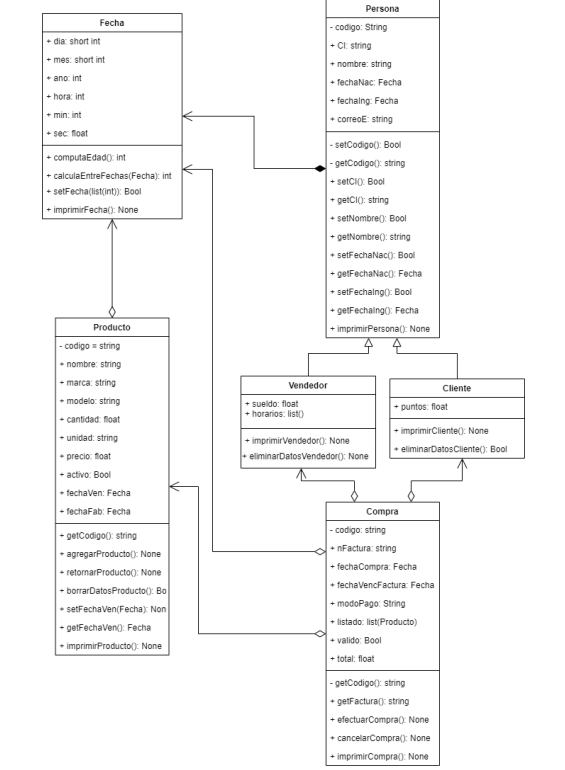
\includegraphics[width=0.5\linewidth]{./anexos/UML INICIAL.png}
    \caption{Diagrama UML inicial}
    \label{fig:umlinicial}
\end{figure}

Para optimizar el sistema se implementó la clase \textit{ItemCompra}, cuya función es encapsular los datos necesarios para calcular el subtotal de una línea de factura. Cada línea almacena el producto, su cantidad y precio unitario, y calcula el monto total multiplicando estos valores. La clase \textit{Compra} obtiene el total sumando todos los \textit{ItemCompra}.  

A su vez, se incorporó la clase \textit{Menu}, encargada de la lógica de interacción con el usuario: gestiona las operaciones de creación, modificación y eliminación sobre las demás clases del sistema, centralizando la interfaz y la recolección de datos.


\item 
\textbf{Código en Python.} Finalizado el diagrama UML, se implementó el código en \textit{Python} aplicando los conceptos de P.O.O. Se incorporaron atributos, métodos, getters y setters necesarios para el funcionamiento de las clases, además de librerías que simplifican su manejo.  

En la clase \textit{Menu} se desarrolló la lógica de navegación que permite al usuario interactuar con el sistema, ofreciendo las siguientes opciones:
\begin{itemize}
    \item Consultar información
    \item Crear información
    \item Borrar información
    \item Menú compras
    \item Salir
\end{itemize}


\item \textbf{Almacenamiento de datos.}
Las listas en memoria se sincronizan con archivos ``.txt'' en formato JSON Lines en \texttt{./db} (\texttt{dbProductos.txt}, \texttt{dbClientes.txt}, \texttt{dbVendedores.txt}, \texttt{dbCompras.txt}). Al iniciar, si el archivo existe se carga como JSONL o arreglo JSON; si no, se parte de listas vacías. El guardado es atómico (\texttt{.tmp} → reemplazo) para evitar corrupciones.  

Las compras se persisten de forma referencial (códigos de cliente, vendedor y productos, cantidades y metadatos) y al cargar se reconstruyen y validan dichas referencias. Véase el ítem “Funciones de lectura y guardado (TXT/JSON Lines)” para más detalle.


\item \textbf{Verificación y validación.}
Se probaron unidades (\texttt{Fecha}, \texttt{Cliente}, \texttt{Vendedor}, \texttt{Producto}, \texttt{ItemCompra} y cálculos de subtotal/total) y luego el flujo integrado con un conjunto mínimo (2 clientes, 2 vendedores, 3 productos y 2 compras), usando \texttt{save\_all("./db", ...)} y posterior recarga.  
Criterios de aceptación:
\begin{itemize}
  \item \texttt{dbClientes.txt}, \texttt{dbVendedores.txt}, \texttt{dbProductos.txt} y \texttt{dbCompras.txt} se generan sin errores.
  \item Las compras se guardan por referencias (códigos y cantidades) y, al recargar, cada código se resuelve a un objeto válido.
  \item Los totales previos al guardado coinciden con los recalculados tras la carga.
  \item Si se fuerza un código inexistente, el sistema lo informa al reconstruir, evitando datos corruptos.
\end{itemize}
Estas pruebas confirmaron que las clases funcionan de forma aislada y, en conjunto con la persistencia, mantienen coherencia con los requisitos.


\subsection{Justificación y Alcance de la Metodología}
El enfoque metodológico se basó en cuatro pilares: diseño, implementación, persistencia y validación. 
Se utilizó \textbf{Google Colab} como entorno de desarrollo por su soporte colaborativo en la nube y \textbf{Python 3.10} por sus capacidades de programación orientada a objetos. 
El almacenamiento se resolvió con \textbf{JSON Lines (JSONL)} en archivos \texttt{.txt}, facilitando la serialización y deserialización de objetos de forma legible y sin dependencias externas.


\subsection{Criterios de Validación}

La validación del sistema se basó en distintos criterios para garantizar confiabilidad y coherencia. 
Se verificó la consistencia de datos en operaciones de creación, guardado y carga de clientes, vendedores, productos y compras, evitando pérdida de información. 
También se comprobó la validez de las relaciones, asegurando que cada \texttt{ItemCompra} refiera a un \texttt{Producto} existente. 
Otro criterio fue el manejo de errores en las entradas, de modo que datos inválidos fueran rechazados sin comprometer la base. 
Finalmente, se revisaron manualmente reportes como \texttt{imprimirCliente} e \texttt{imprimirCompra}, confirmando que la salida coincidiera con los datos ingresados.


\subsection{Limitaciones}

La metodología presenta algunas limitaciones consideradas como oportunidades de mejora. 
En primer lugar, no se implementaron pruebas unitarias automatizadas, por lo que la validación fue manual y con menor alcance. 
Además, la persistencia en archivos JSONL resulta adecuada para un entorno académico y de pequeña escala, pero no es escalable para grandes volúmenes de datos o accesos concurrentes. 
Por último, el manejo de errores se limita a validaciones básicas de entrada, sin cubrir casos más complejos como concurrencia o corrupción de archivos.

\subsection{Conexión con los Objetivos}

Finalmente, la metodología descrita asegura cumplir con los objetivos planteados al garantizar:
\begin{itemize}
    \item Un modelo UML completo y consistente.
    \item Una implementación funcional en Python siguiendo principios de POO.
    \item Persistencia de datos simple y confiable mediante archivos JSONL.
    \item Validación del correcto funcionamiento a través de casos de prueba controlados.
\end{itemize}
\end{enumerate}



\section{Resultados}\label{sec:resultados}

\subsection{Nuevo UML}

\begin{figure}[H]
    \centering
    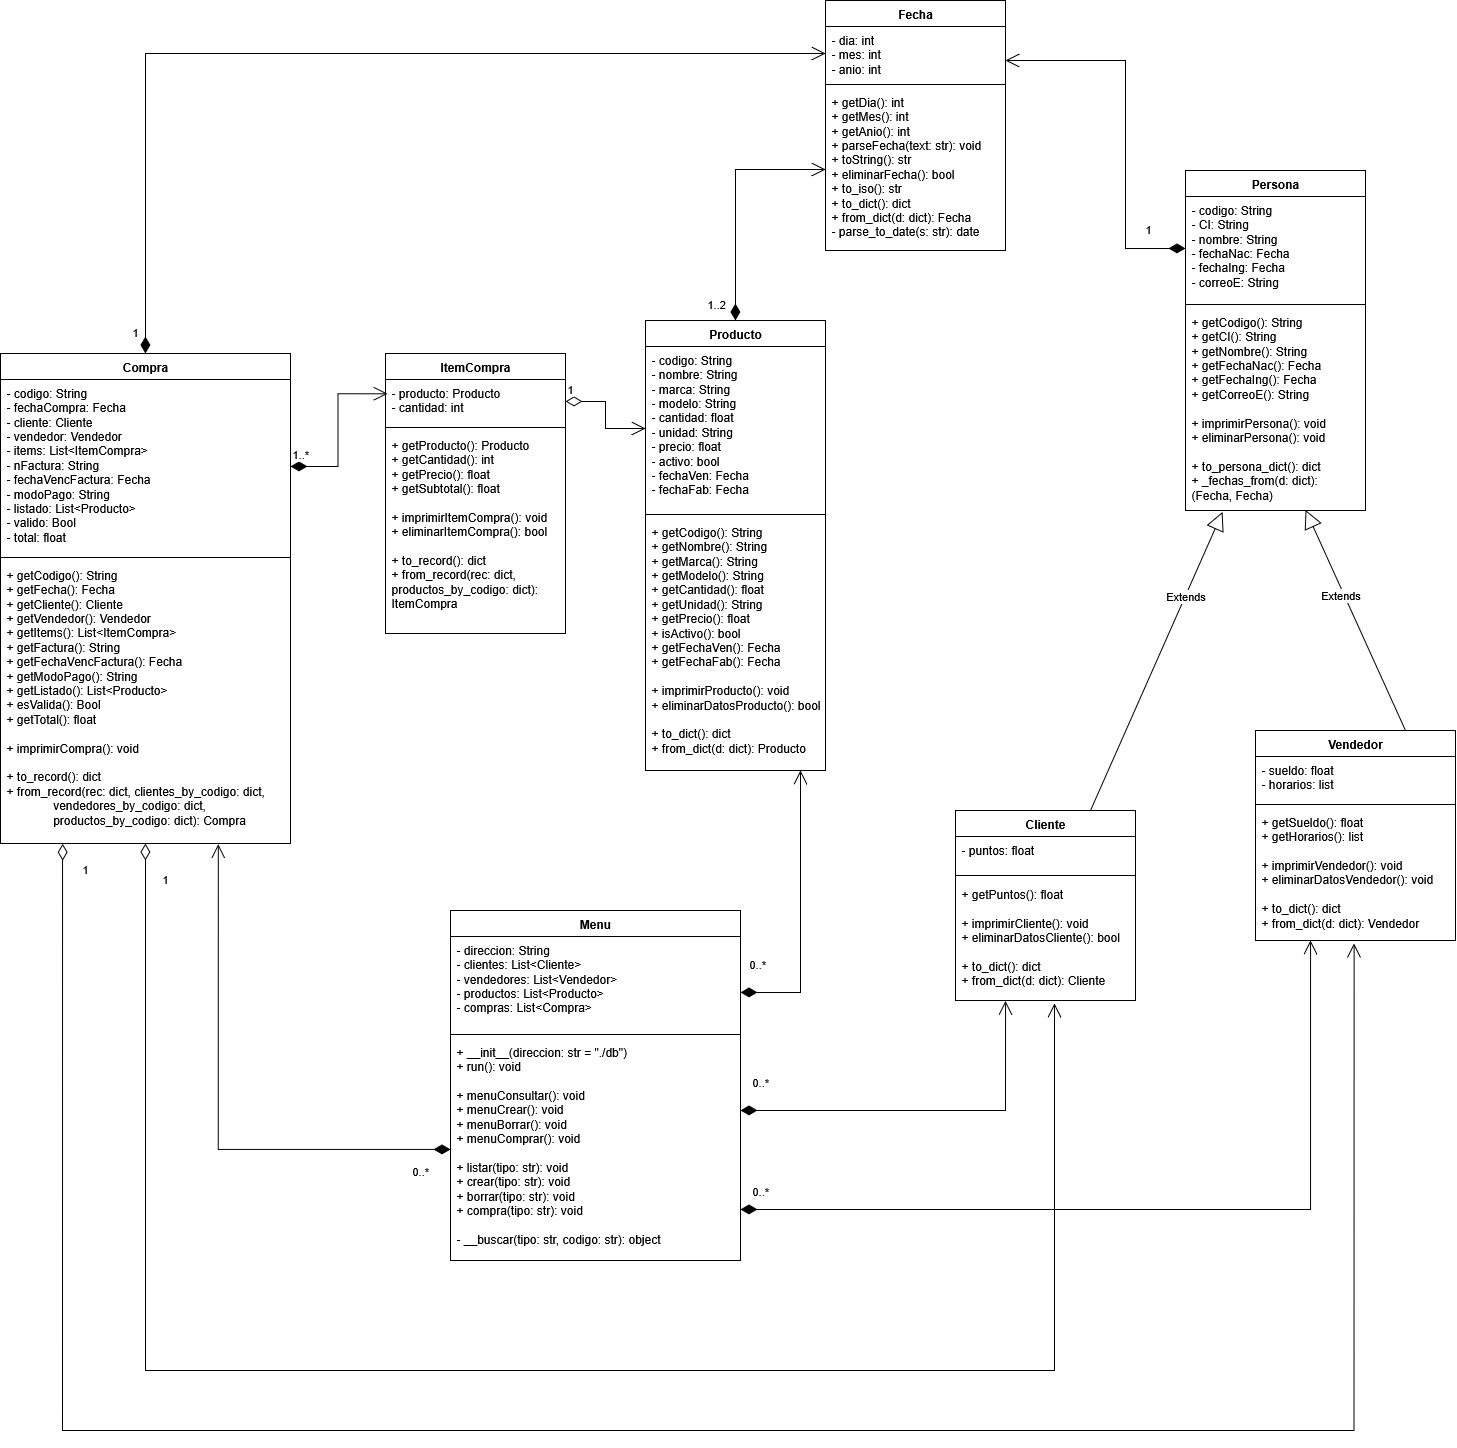
\includegraphics[width=0.84\linewidth]{./anexos/Diagrama UML Final.jpg}
    \caption{Diagrama UML final. Fuente: Elaboración própia}
    \label{fig:umlfinal}
\end{figure}

\paragraph{Cambios respecto al UML inicial.}
En el diagrama final, \texttt{Persona} quedó como clase base, de la cual heredan \texttt{Cliente} y \texttt{Vendedor}, evitando duplicar atributos como código, CI, fechas y correo. 
\texttt{Producto} se amplió con marca, modelo, unidad, estado (activo) y fechas de fabricación y vencimiento, describiendo mejor el inventario.  

\texttt{Compra} pasó a ser el núcleo: además de fecha, cliente, vendedor e ítems, incorpora número de factura, modo de pago, un listado explícito de productos, estado y total. 
Para ello, \texttt{ItemCompra} actúa como vínculo entre compra y producto, con cantidad y subtotal.  

Finalmente, se añadió \texttt{Menu} como interfaz principal, responsable de orquestar las operaciones y conectar con la persistencia en archivos. 
En conjunto, el UML final refleja con mayor fidelidad la implementación y permite futuras extensiones sin afectar la estructura existente.



\subsection{Clases}

El sistema se estructuró siguiendo los principios de la Programación Orientada a Objetos (POO), organizando la lógica en distintas clases que modelan tanto las entidades del dominio como las operaciones del sistema.  
De forma resumida:

\begin{itemize}
    \item \textbf{Fecha}: encapsula día, mes y año, empleado en nacimientos, ingresos y compras.  
    \item \textbf{Persona}: clase base con atributos comunes a \texttt{Cliente} y \texttt{Vendedor}.  
    \item \textbf{Cliente} y \textbf{Vendedor}: subclases de \texttt{Persona} con atributos propios, como puntos acumulados o sueldo y horarios.  
    \item \textbf{Producto}: describe los artículos a vender, con identificación, stock y fechas de fabricación y vencimiento.  
    \item \textbf{ItemCompra}: vincula un producto con una cantidad, formando parte de una compra.  
    \item \textbf{Compra}: centraliza la transacción, integrando cliente, vendedor, productos, fecha, factura y total.  
    \item \textbf{Menu}: gestiona la interacción con el usuario y el flujo de operaciones, incluida la compra.
\end{itemize}



\subsection{Guardado y lectura de archivos}

La persistencia se implementó con archivos de texto en formato \texttt{JSON Lines} (JSONL), donde cada objeto se almacena en una línea independiente. Esto facilita la lectura secuencial, la compatibilidad con distintos lenguajes y la inspección manual.  

Para el \textbf{guardado}, la función \texttt{save\_all} recorre las listas de \texttt{Cliente}, \texttt{Vendedor}, \texttt{Producto} y \texttt{Compra}, serializando cada objeto con \texttt{to\_dict} o \texttt{to\_record}. Luego, \texttt{\_write\_jsonl\_atomic} escribe en un archivo temporal (\texttt{.tmp}) y lo reemplaza de forma atómica, evitando corrupciones en caso de error.  

En la \textbf{lectura}, \texttt{\_read\_jsonl} interpreta cada línea como JSON y devuelve una lista de diccionarios. A partir de ellos, las funciones \texttt{load\_clientes}, \texttt{load\_vendedores}, \texttt{load\_productos} y \texttt{load\_compras} reconstruyen las instancias mediante \texttt{from\_dict} o \texttt{from\_record}. En \texttt{Compra}, además, se valida la integridad referencial verificando que cada ítem apunte a un \texttt{Producto}, \texttt{Cliente} y \texttt{Vendedor} cargados previamente.


Este mecanismo asegura:
\begin{itemize}
    \item Integridad de datos al manipular listas de objetos entre sesiones.
    \item Independencia del sistema frente a gestores de bases de datos externos.
    \item Sencillez en la depuración y validación de archivos.
\end{itemize}

En la Figura~\ref{fig:jsonl} se muestra un ejemplo de registro almacenado en el archivo \texttt{dbCompras.txt}, donde se observa la referencia a códigos de cliente, vendedor y productos.

\begin{figure}[H]
    \centering
    \begin{lstlisting}[language=Python]
        {"cliente_codigo": "", "codigo": "C01", "fecha": "1990-01-01", "fechaVencFactura": "2024-04-20", "items": [{"cantidad": 2, "producto_codigo": ""}, {"cantidad": 10, "producto_codigo": "P01"}, {"cantidad": 20, "producto_codigo": "P02"}], "listado": ["", "P01", "P02"], "modoPago": "Tarjeta", "nFactura": "F001", "total": 11009.2, "valido": true, "vendedor_codigo": ""}
    \end{lstlisting}
    \caption{Ejemplo de registro en formato JSONL para una compra.}
    \label{fig:jsonl}
\end{figure}

\subsection{Resumen de validaciones}
\begin{table}[H]\centering
\begin{tabular}{p{8cm} c p{6cm}}
\toprule
\textbf{Criterio} & \textbf{Estado} & \textbf{Evidencia} \\
\midrule
Archivos \texttt{db*.txt} generados sin errores &
\textbf{OK} &
Logs de ejecución y archivos en \texttt{./db} \\
Compras por referencias y reconstrucción correcta &
\textbf{OK} &
Carga con \texttt{load\_compras} (IDs válidos) \\
Totales antes/después del guardado coinciden &
\textbf{OK} &
Comparación de \texttt{getTotal()} vs recálculo \\
Referencias inválidas se reportan sin romper datos &
\textbf{OK} &
Mensajes de advertencia y omisión controlada \\
\bottomrule
\end{tabular}
\caption{Criterios de validación y resultados.}
\end{table}



% --- Evidencias ---






\section{Conclusiones} El proyecto logró implementar un modelo de dominio coherente en POO con clases bien delimitadas (\texttt{Persona}, \texttt{Cliente}, \texttt{Vendedor}, \texttt{Producto}, \texttt{ItemCompra}, \texttt{Compra} y \texttt{Menu}), reflejado en un UML final consistente con las decisiones de diseño. La separación entre lógica de negocio y persistencia permitió serializar y rehidratar objetos de forma confiable usando JSON Lines, con escritura atómica para evitar corrupción y diccionarios–índice para preservar la integridad referencial y mejorar el rendimiento en accesos y cargas. Desde el punto de vista técnico, el sistema demostró que con un conjunto acotado de patrones (encapsulamiento, composición de \texttt{Compra}–\texttt{ItemCompra}, asociaciones con \texttt{Cliente}/\texttt{Vendedor} y normalización de fechas) es posible obtener un flujo completo: alta, listado, borrado, compra y posterior relectura desde disco, manteniendo coherencia de datos y un contrato claro de métodos públicos. La experiencia de uso mejoró gracias a validaciones simples de entrada y a una impresión estandarizada de entidades, lo que facilitó la verificación manual. También quedaron visibles límites razonables: la ausencia de pruebas unitarias automatizadas, el uso de archivos de texto como única capa de persistencia y la falta de control de concurrencia. Estas restricciones no afectan el objetivo del laboratorio, pero marcan un camino de evolución: migrar a una base de datos ligera, incorporar tests para casos borde (referencias inexistentes, formatos de fecha irregulares, cantidades inválidas), y agregar reglas de negocio como descuentos, impuestos y manejo de stock con entradas/salidas. En síntesis, se cumplió el objetivo de modelar, implementar y persistir el dominio propuesto con una arquitectura simple, extensible y didáctica. El diseño actual deja el terreno preparado para crecer sin romper interfaces: la capa de datos es intercambiable, las entidades están encapsuladas y el UML captura las relaciones esenciales que guían futuras ampliaciones.

\newpage

\bibliographystyle{alpha}
\nocite{*}
\bibliography{referencias.bib}


\newpage

\appendix

\section{Recursos}

\begin{itemize}
  \item \textbf{Carpeta general (Drive):}
    \href{https://drive.google.com/drive/folders/1nIY4LP34ZPg8fk4kJ2LFdMDJ417Zf3oI}
         {\nolinkurl{https://drive.google.com}}
  \item \textbf{Diagrama UML:}
    \href{https://drive.google.com/file/d/17fj9S_zEiaoR2zrMGGmN1JwGT5Dy9nQF}
         {\nolinkurl{https://drive.google.com}}
  \item \textbf{Código (Google Colab):}
    \href{https://colab.research.google.com/drive/1onQJxx9BtXw5OUwlhw7OiUK88e6yWuuB}
         {\nolinkurl{https://colab.research.google.com}}
  \item \textbf{Documento (Google Docs):}
    \href{https://docs.google.com/document/d/1KQ9onM5Ge5rgCczQMDyyks0Ff6jJonFbX9TXnuF9RjE}
         {\nolinkurl{https://docs.google.com}}
  \item \textbf{Overleaf / coordinación:}
    \href{https://www.overleaf.com/project/68d4487b8e93ecf1153e9b87}
         {\nolinkurl{https://www.overleaf.com/}}
\end{itemize}

\section{CÓDIGO-FUENTE EN LENGUAJE PYTHON}

\lstinputlisting[language=python]{anexos/codigo.py}

\section{EVIDENCIAS DE FUNCIONAMIENTO}

\begin{multicols}{2}
\centering

\begin{figure}[H]
    \centering
    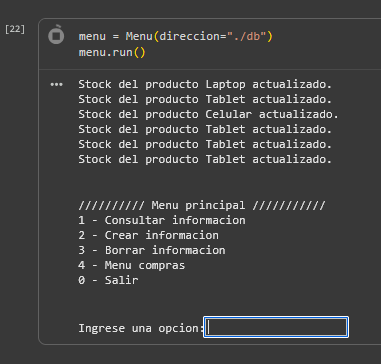
\includegraphics[width=0.5\linewidth]{./anexos/evidencias/menuPrincipal.png}
    \caption{Menú principal}
    \label{fig:menuPrincipal}
\end{figure}

\begin{figure}[H]
    \centering
    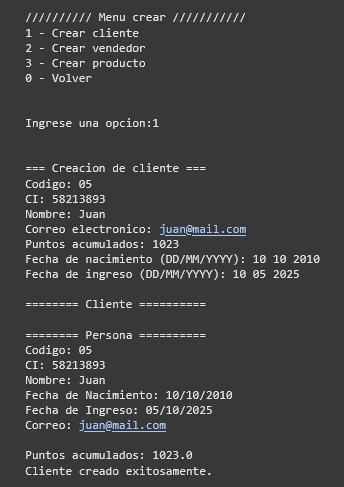
\includegraphics[width=0.5\linewidth]{./anexos/evidencias/crearCliente.png}
    \caption{Creación de cliente}
    \label{fig:crearCliente}
\end{figure}

\begin{figure}[H]
    \centering
    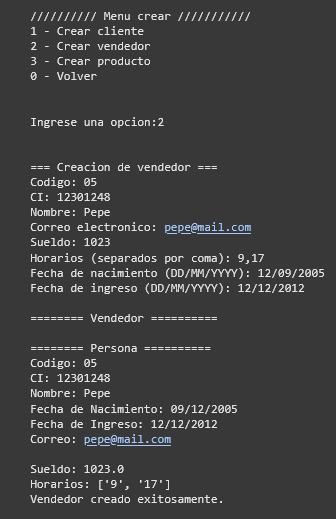
\includegraphics[width=0.5\linewidth]{./anexos/evidencias/crearVendedor.png}
    \caption{Creación de vendedor}
    \label{fig:crearVendedor}
\end{figure}

\begin{figure}[H]
    \centering
    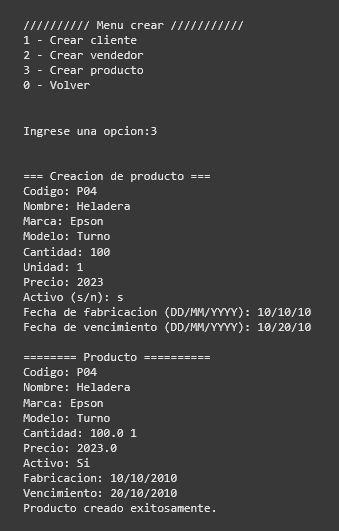
\includegraphics[width=0.5\linewidth]{./anexos/evidencias/crearProducto.png}
    \caption{Creación de producto}
    \label{fig:crearProducto}
\end{figure}

\begin{figure}[H]
    \centering
    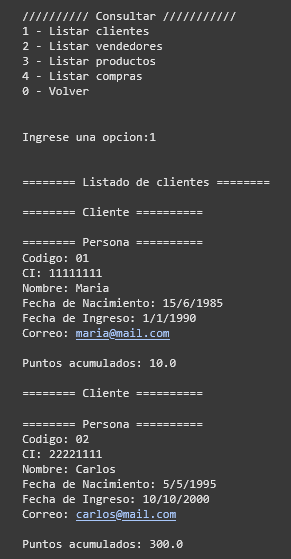
\includegraphics[width=0.5\linewidth]{./anexos/evidencias/listadoClientes.png}
    \caption{Listado de clientes}
    \label{fig:listadoClientes}
\end{figure}

\begin{figure}[H]
    \centering
    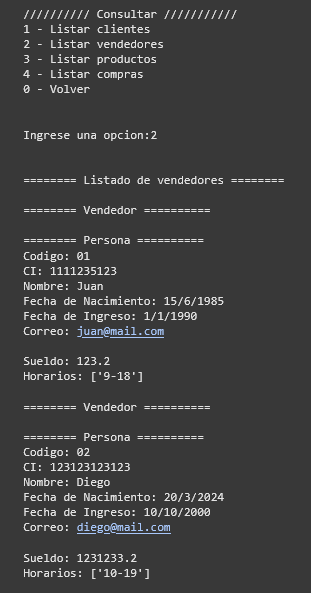
\includegraphics[width=0.5\linewidth]{./anexos/evidencias/listadoVendedores.png}
    \caption{Listado de vendedores}
    \label{fig:listadoVendedores}
\end{figure}

\begin{figure}[H]
    \centering
    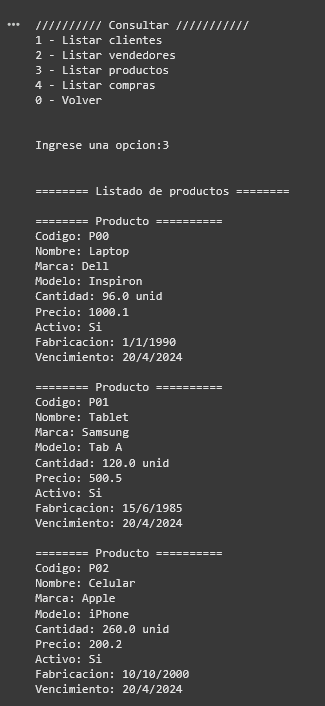
\includegraphics[width=0.5\linewidth]{./anexos/evidencias/listadoProductos.png}
    \caption{Listado de productos}
    \label{fig:listadoProductos}
\end{figure}

\begin{figure}[H]
    \centering
    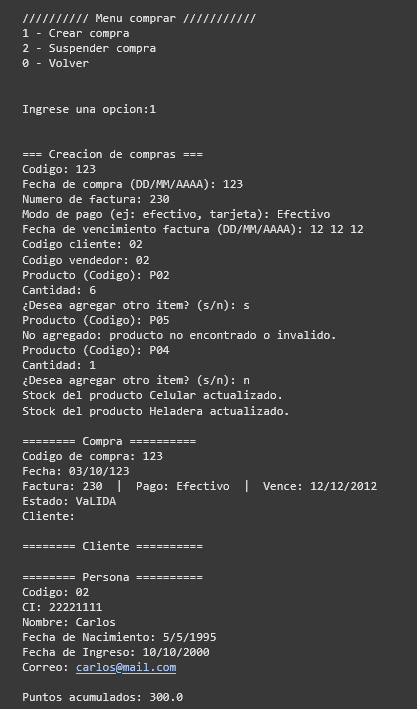
\includegraphics[width=0.5\linewidth]{./anexos/evidencias/crearCompra1.png}
    \caption{Creación de compra (paso 1)}
    \label{fig:crearCompra1}
\end{figure}

\begin{figure}[H]
    \centering
    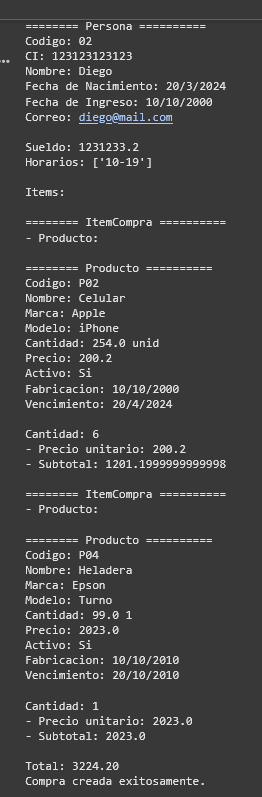
\includegraphics[width=0.5\linewidth]{./anexos/evidencias/crearCompra2.png}
    \caption{Creación de compra (paso 2)}
    \label{fig:crearCompra2}
\end{figure}

\begin{figure}[H]
    \centering
    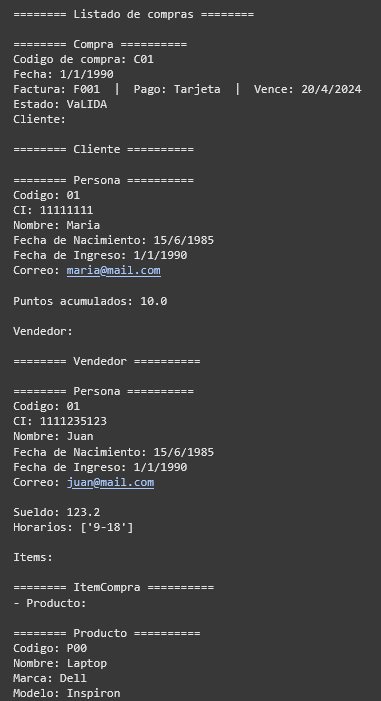
\includegraphics[width=0.5\linewidth]{./anexos/evidencias/listadoCompra.png}
    \caption{Listado de compras}
    \label{fig:listadoCompra}
\end{figure}

\begin{figure}[H]
    \centering
    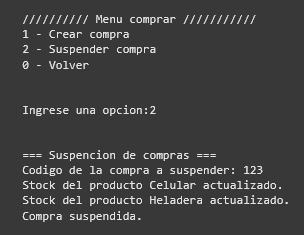
\includegraphics[width=0.5\linewidth]{./anexos/evidencias/suspenderCompra.png}
    \caption{Suspensión de compra}
    \label{fig:suspenderCompra}
\end{figure}

\begin{figure}[H]
    \centering
    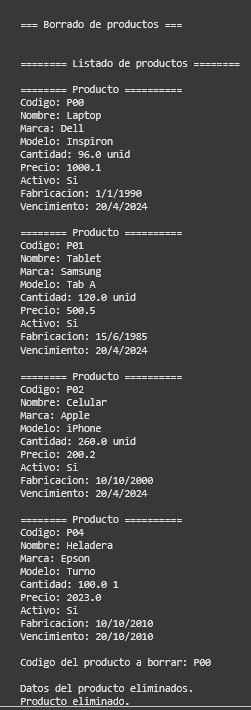
\includegraphics[width=0.5\linewidth]{./anexos/evidencias/borrarProducto.png}
    \caption{Borrado de producto}
    \label{fig:borrarProducto}
\end{figure}

\begin{figure}[H]
    \centering
    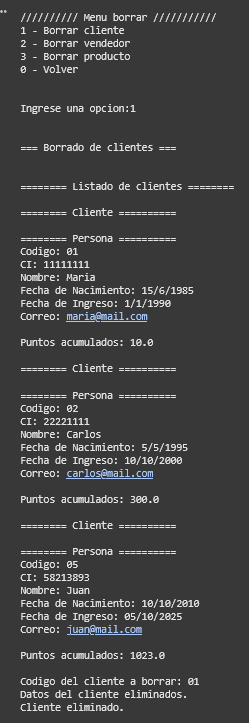
\includegraphics[width=0.5\linewidth]{./anexos/evidencias/eliminarCliente.png}
    \caption{Borrado de cliente}
    \label{fig:eliminarCliente}
\end{figure}

\begin{figure}[H]
    \centering
    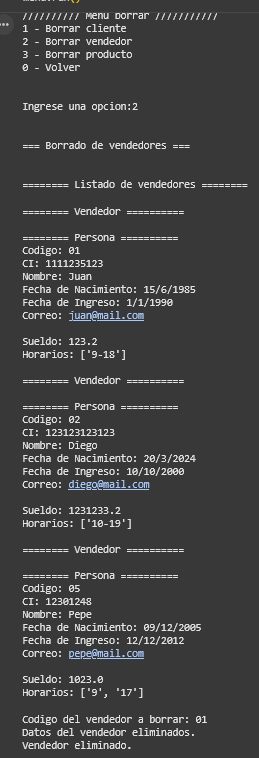
\includegraphics[width=0.5\linewidth]{./anexos/evidencias/eliminarVendedor.png}
    \caption{Borrado de vendedor}
    \label{fig:eliminarVendedor}
\end{figure}

\end{multicols}

\newpage

\section{RESULTADOS EN ARCHIVOS .TXT}

\lstinputlisting{anexos/evidencias/dbClientes.txt}
\lstinputlisting{anexos/evidencias/dbCompras.txt}
\lstinputlisting{anexos/evidencias/dbVendedores.txt}
\lstinputlisting{anexos/evidencias/dbProductos.txt}


\end{document}
